\documentclass{dit}

\usepackage{amsmath}
\usepackage{hyperref}
\pdfstringdefDisableCommands{\def\_{_}}
\usepackage{tikz}
% \usepackage{pgfplots}

% allow embedding files in the PDF so viewers can open/save them
\usepackage{attachfile2}

% CSV import for tables
\usepackage{csvsimple}
\usepackage{longtable}
% ensure floats appear before section text when desired
\usepackage{placeins}
% code/listing support for run commands
\usepackage{listings}
\lstset{basicstyle=\ttfamily\small,breaklines=true,columns=fullflexible}

% Macro to show how to run binaries in a consistent way
\newcommand{\runcmd}[1]{\vspace{6pt}\noindent\textbf{Run: }\lstinline!#1!\par}

\usepackage[english,greek]{babel}
% helper to typeset short English fragments when main language is Greek
\newcommand{\en}[1]{\foreignlanguage{english}{#1}}

\newcommand*{\name}{Ευάγγελος Τραϊκόγλου}
\newcommand*{\id}{1115202200189}
\newcommand*{\course}{Παράλληλα Συστήματα}
\newcommand*{\assignment}{Εργασία \en{Mpi}}

\begin{document}

\maketitle

% \tableofcontents
\begin{itemize}
    \item \en{cpu}: \en{i5-6500}
    \item \en{cores}: \en{4 physical}
    \item \en{os, kernel}: \en{Ubuntu 20.04.6 LTS, 5.4.0-216-generic}
    \item \en{comp version}: \en{gcc 9.4.0}
\end{itemize}

\underline{Σημείωση}: 
Εκτός της 3ης άσκησης, όλα τα πειράματα τρέξαν με ένα αρχείο όπου όριζε 4 διαθέσιμα \en{slots} 
(αφού τα \en{linux} διαθέτουν 4 πυρήνες ανά \en{cpu} και όχι \en{hyperthreading}) σε όλα
τα μηχανήματα, εκτός του \en{linux03} που δεν ήταν διαθέσιμο. Δηλαδή η εντολή ήταν: 
\\
\en{\runcmd{mmpiexec -f machines -n <num of proc> ...}}
Επιπλέον, μικρές αποκλίσεις που μπορεί να παρατηρούνται από το επιθυμητό αποτέλεσμα οφείλονται στη χρήση διαμοιραζόμενων
υπολογιστικών πόρων. Αυτό αν φαίνεται, συνήθως πλήττει τα αποτελέσματα όπου το \en{n} είναι μεγάλο και 
εμπλέκονται πολλά μηχανήματα.

\section{\en{Polynomial Multiplication}}
Η πρώτη άσκηση επικεντρώνεται στον πολλαπλασιασμό πολυωνύμων βαθμού \en{n}.
Ο σειριακός αλγόριθμος ακολουθεί την απλή υλοποίηση $\mathcal{O}(n^2)$ χρόνου και τρέχει μόνο από την
διεργασία 0.
Στον παράλληλο, η διεργασία 0 αρχικοποιεί τα πολυώνυμα και τις δομές που χρειάζονται. Κάθε διεργασία υπολογίζει
ένα μέρος του τελικού πολυωνύμου πολλαπλασιάζοντας ένα μέρος του \en{pol1} με ολόκληρο το \en{pol2}. Άρα το \en{pol2}
γίνεται \en{broadcast} και το \en{pol1} \en{Scatterv} (καθώς το μέγεθος του \en{pol1} μπορεί να μη διαιρείται ακριβώς με
το \en{num\_proc}). Το αποτέλεσμα συγκεντρώνεται μέσω της \en{Reduce} στη διεργασία 0. Το \en{local result array} κρατά
μερικό άθροισμα των συντελεστών του τελικού πολυωνύμου (\en{rank == 0} $(A_0 .. A_k) \cdot (B_0 .. B_n)$, 
\en{rank == 1} $(A_{k+1} .. A_2k) \cdot (B_0 .. B_n)$, ...) και η \en{Reduce} παίρνει τα μερικά αθροίσματα σε κάθε θέση
του \en{local} τελικού πολυωνύμου και τα αθροίζει και αποθηκεύει στη κατάλληλη θέση στο τελικό πολυώνυμο στην διεργασία 0.
\\
\en{\runcmd{mpiexec -n <nodes> ./polynomial_mult -n <degree>}}

\underline{Σημείωση}: 
Όλα τα πειράματα υπάρχουν στα \en{csv} αρχεία: \en{mpi\_pol\_results.csv}, \en{comparison\_mpi\_vs\_omp.csv}.

\begin{figure}[htbp]
    \centering
    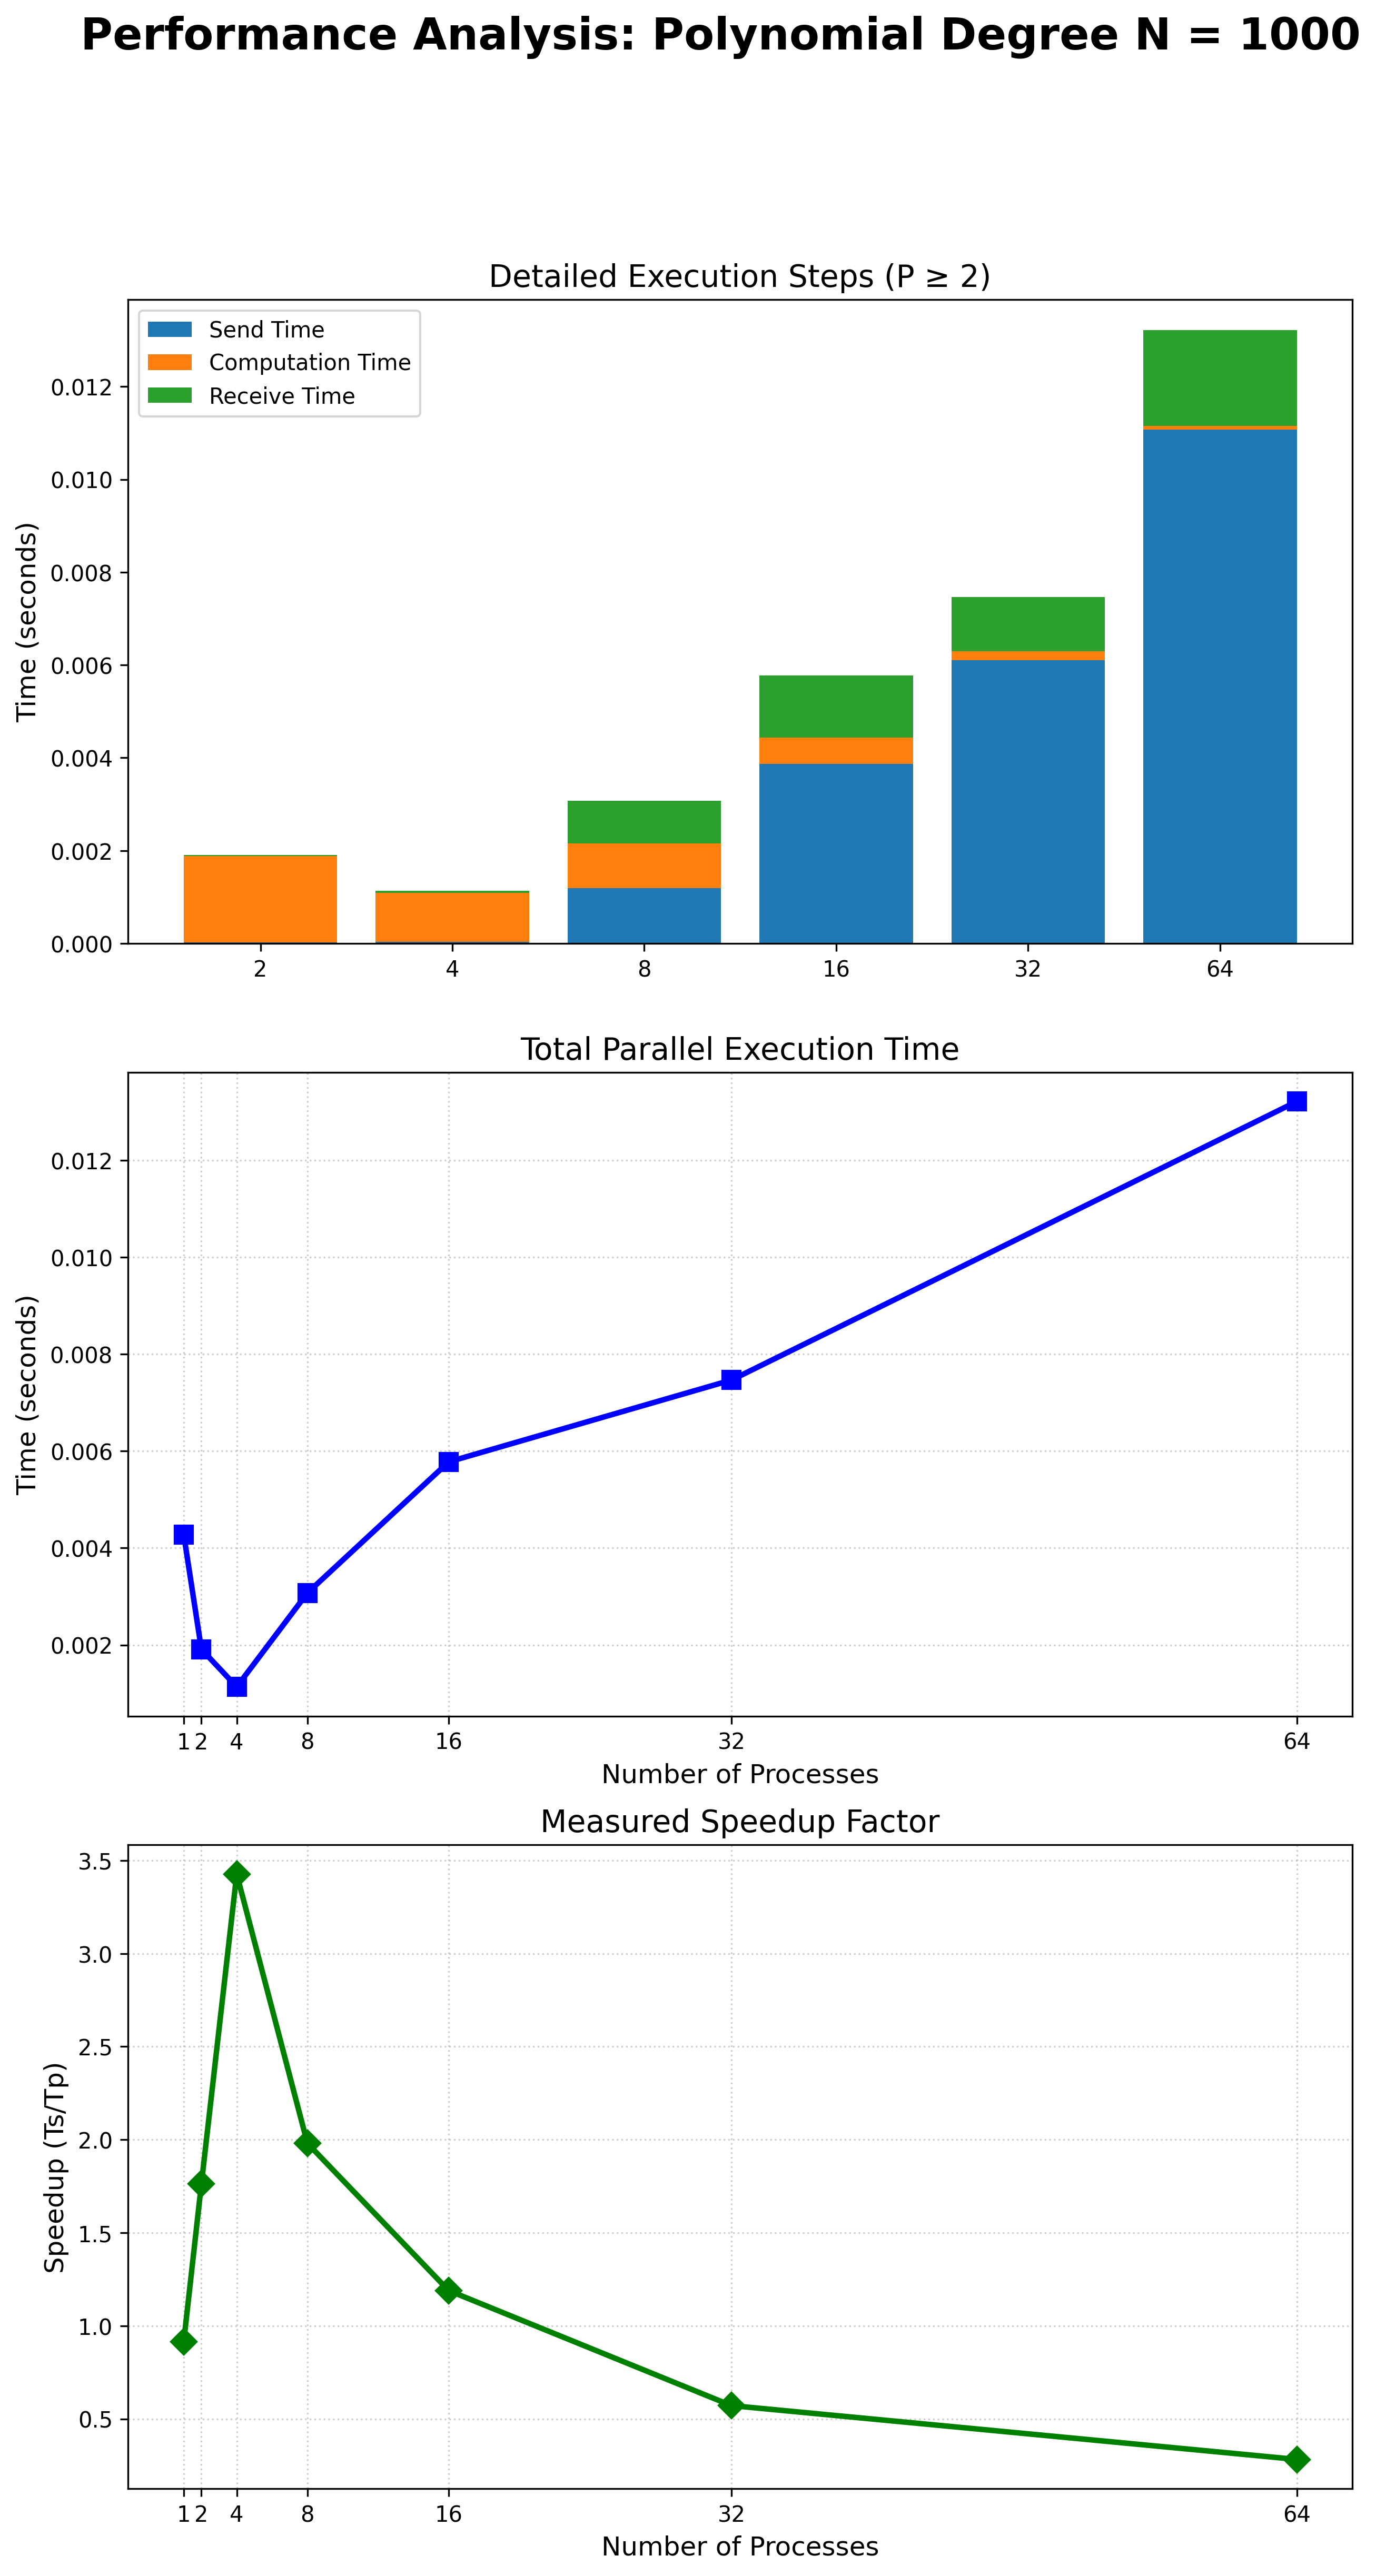
\includegraphics[width=0.8\linewidth]{graphs/pol_mult_N1000.png}
\end{figure}


\begin{figure}[htbp]
    \centering
    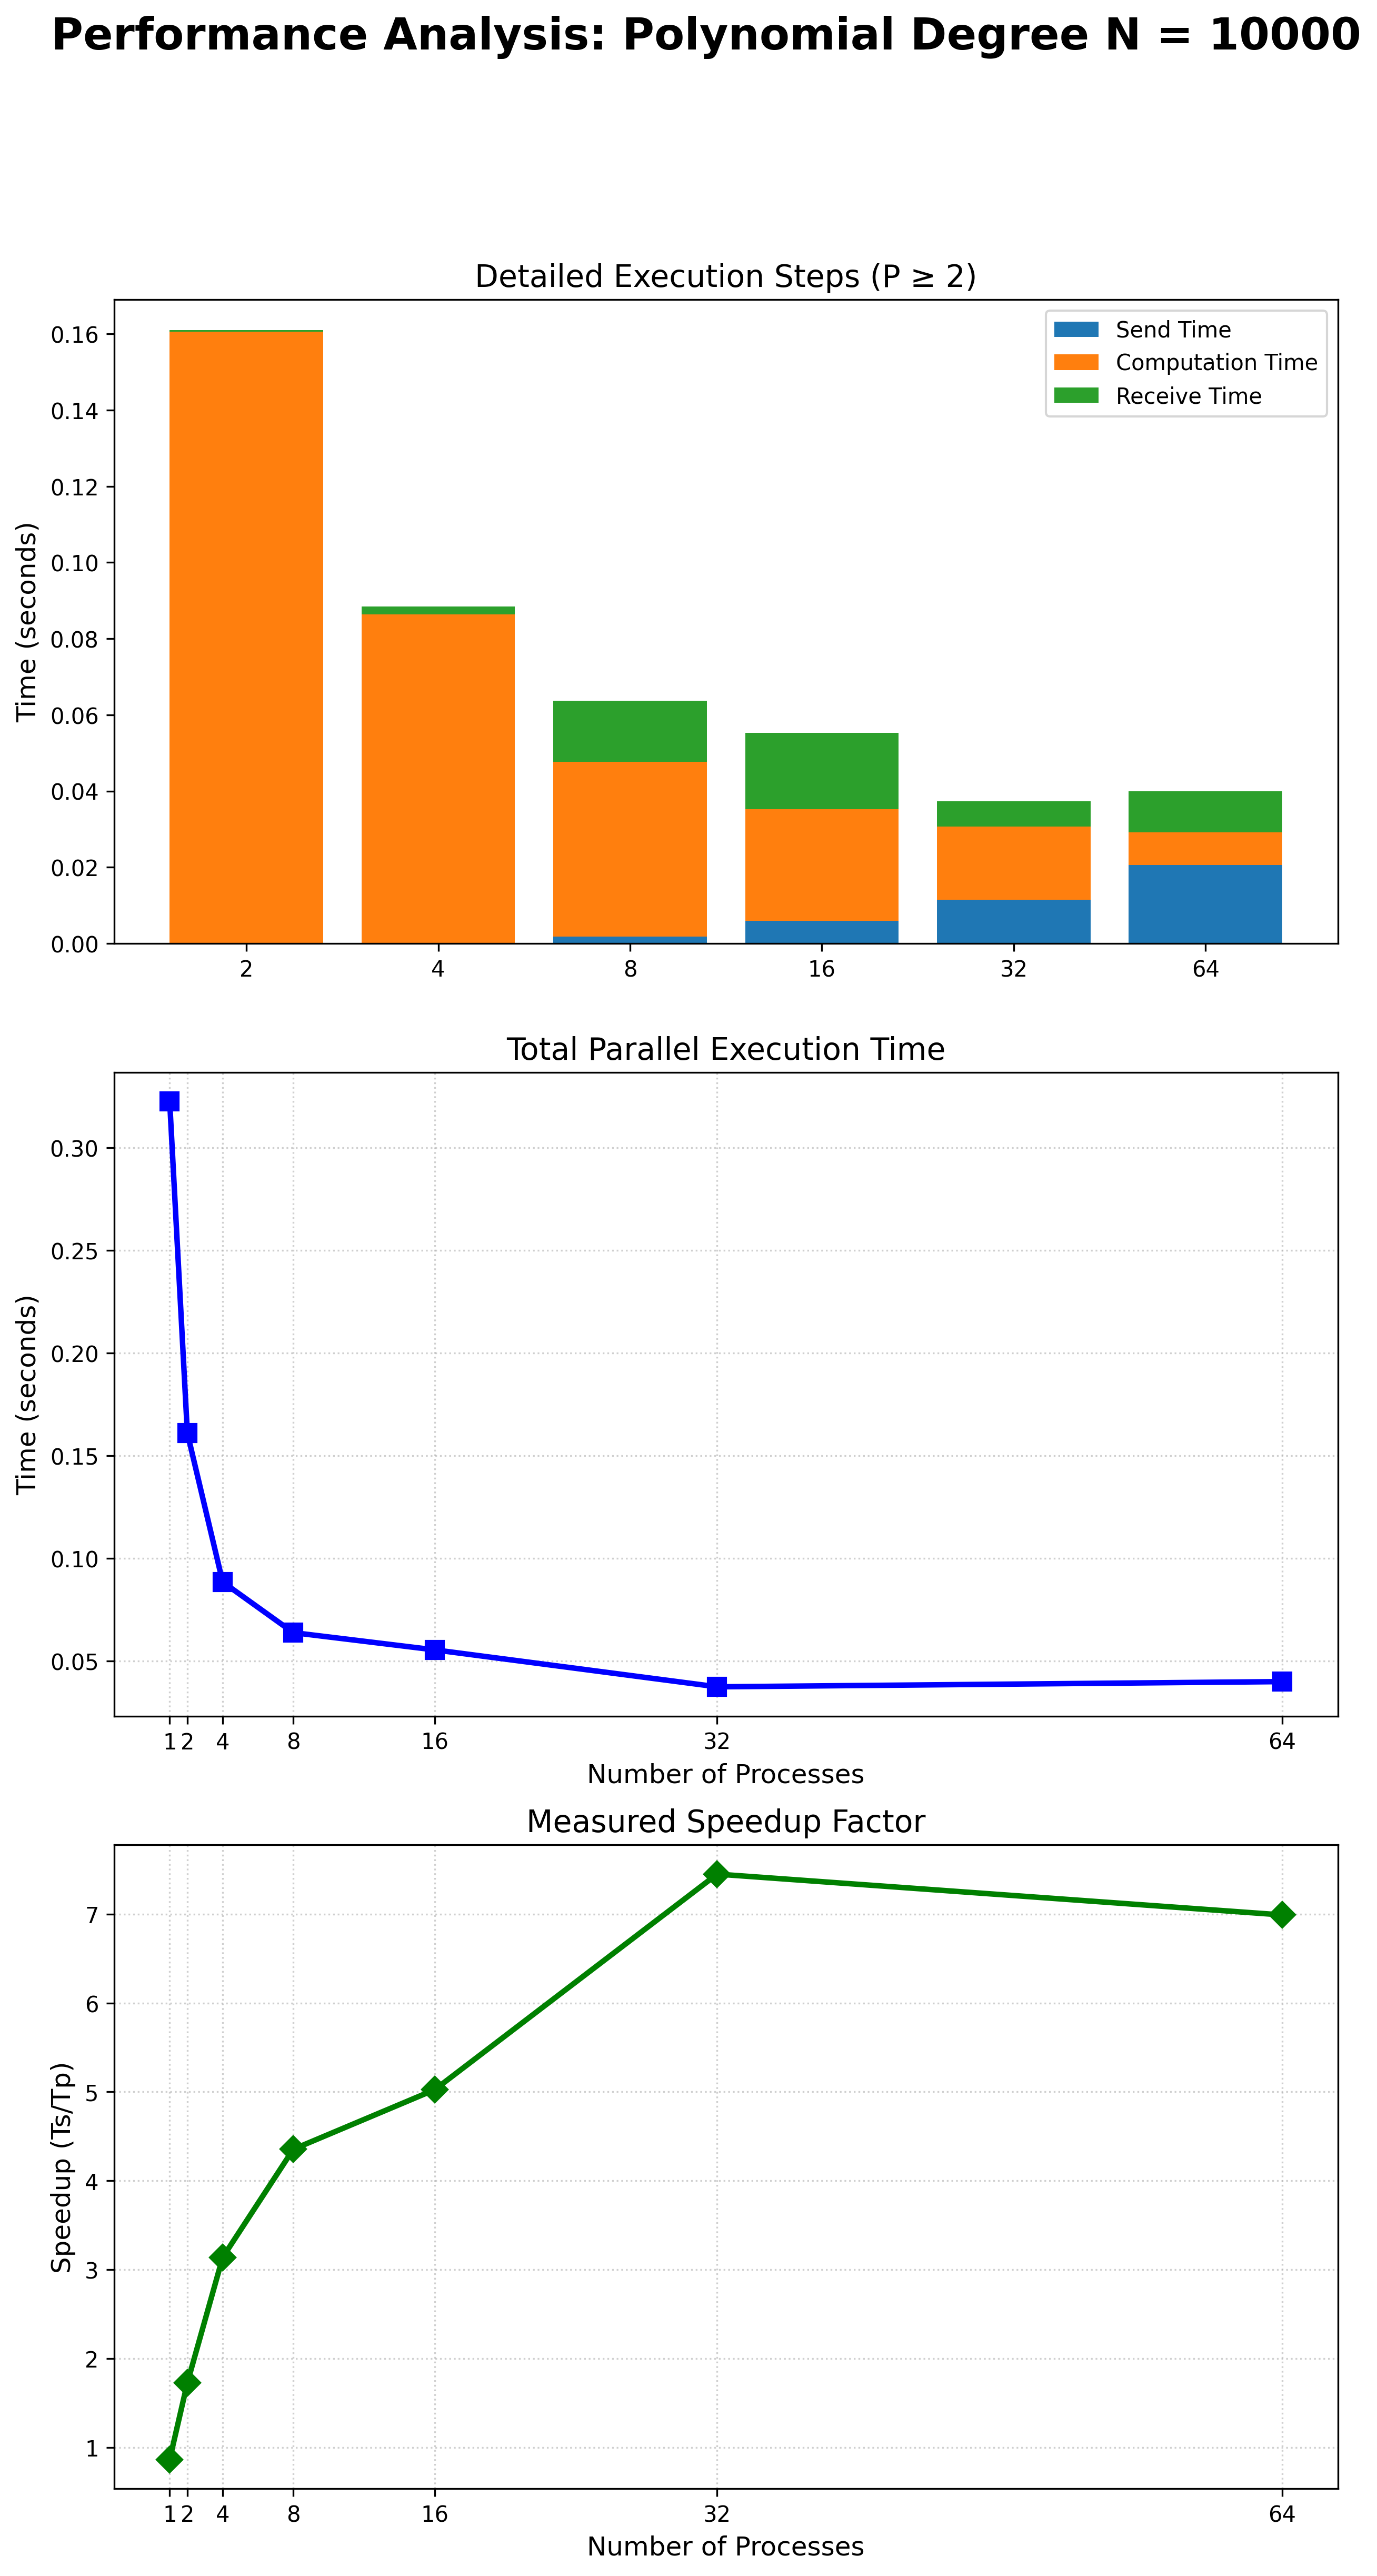
\includegraphics[width=0.8\linewidth]{graphs/pol_mult_N10000.png}
\end{figure}

\begin{figure}[htbp]
    \centering
    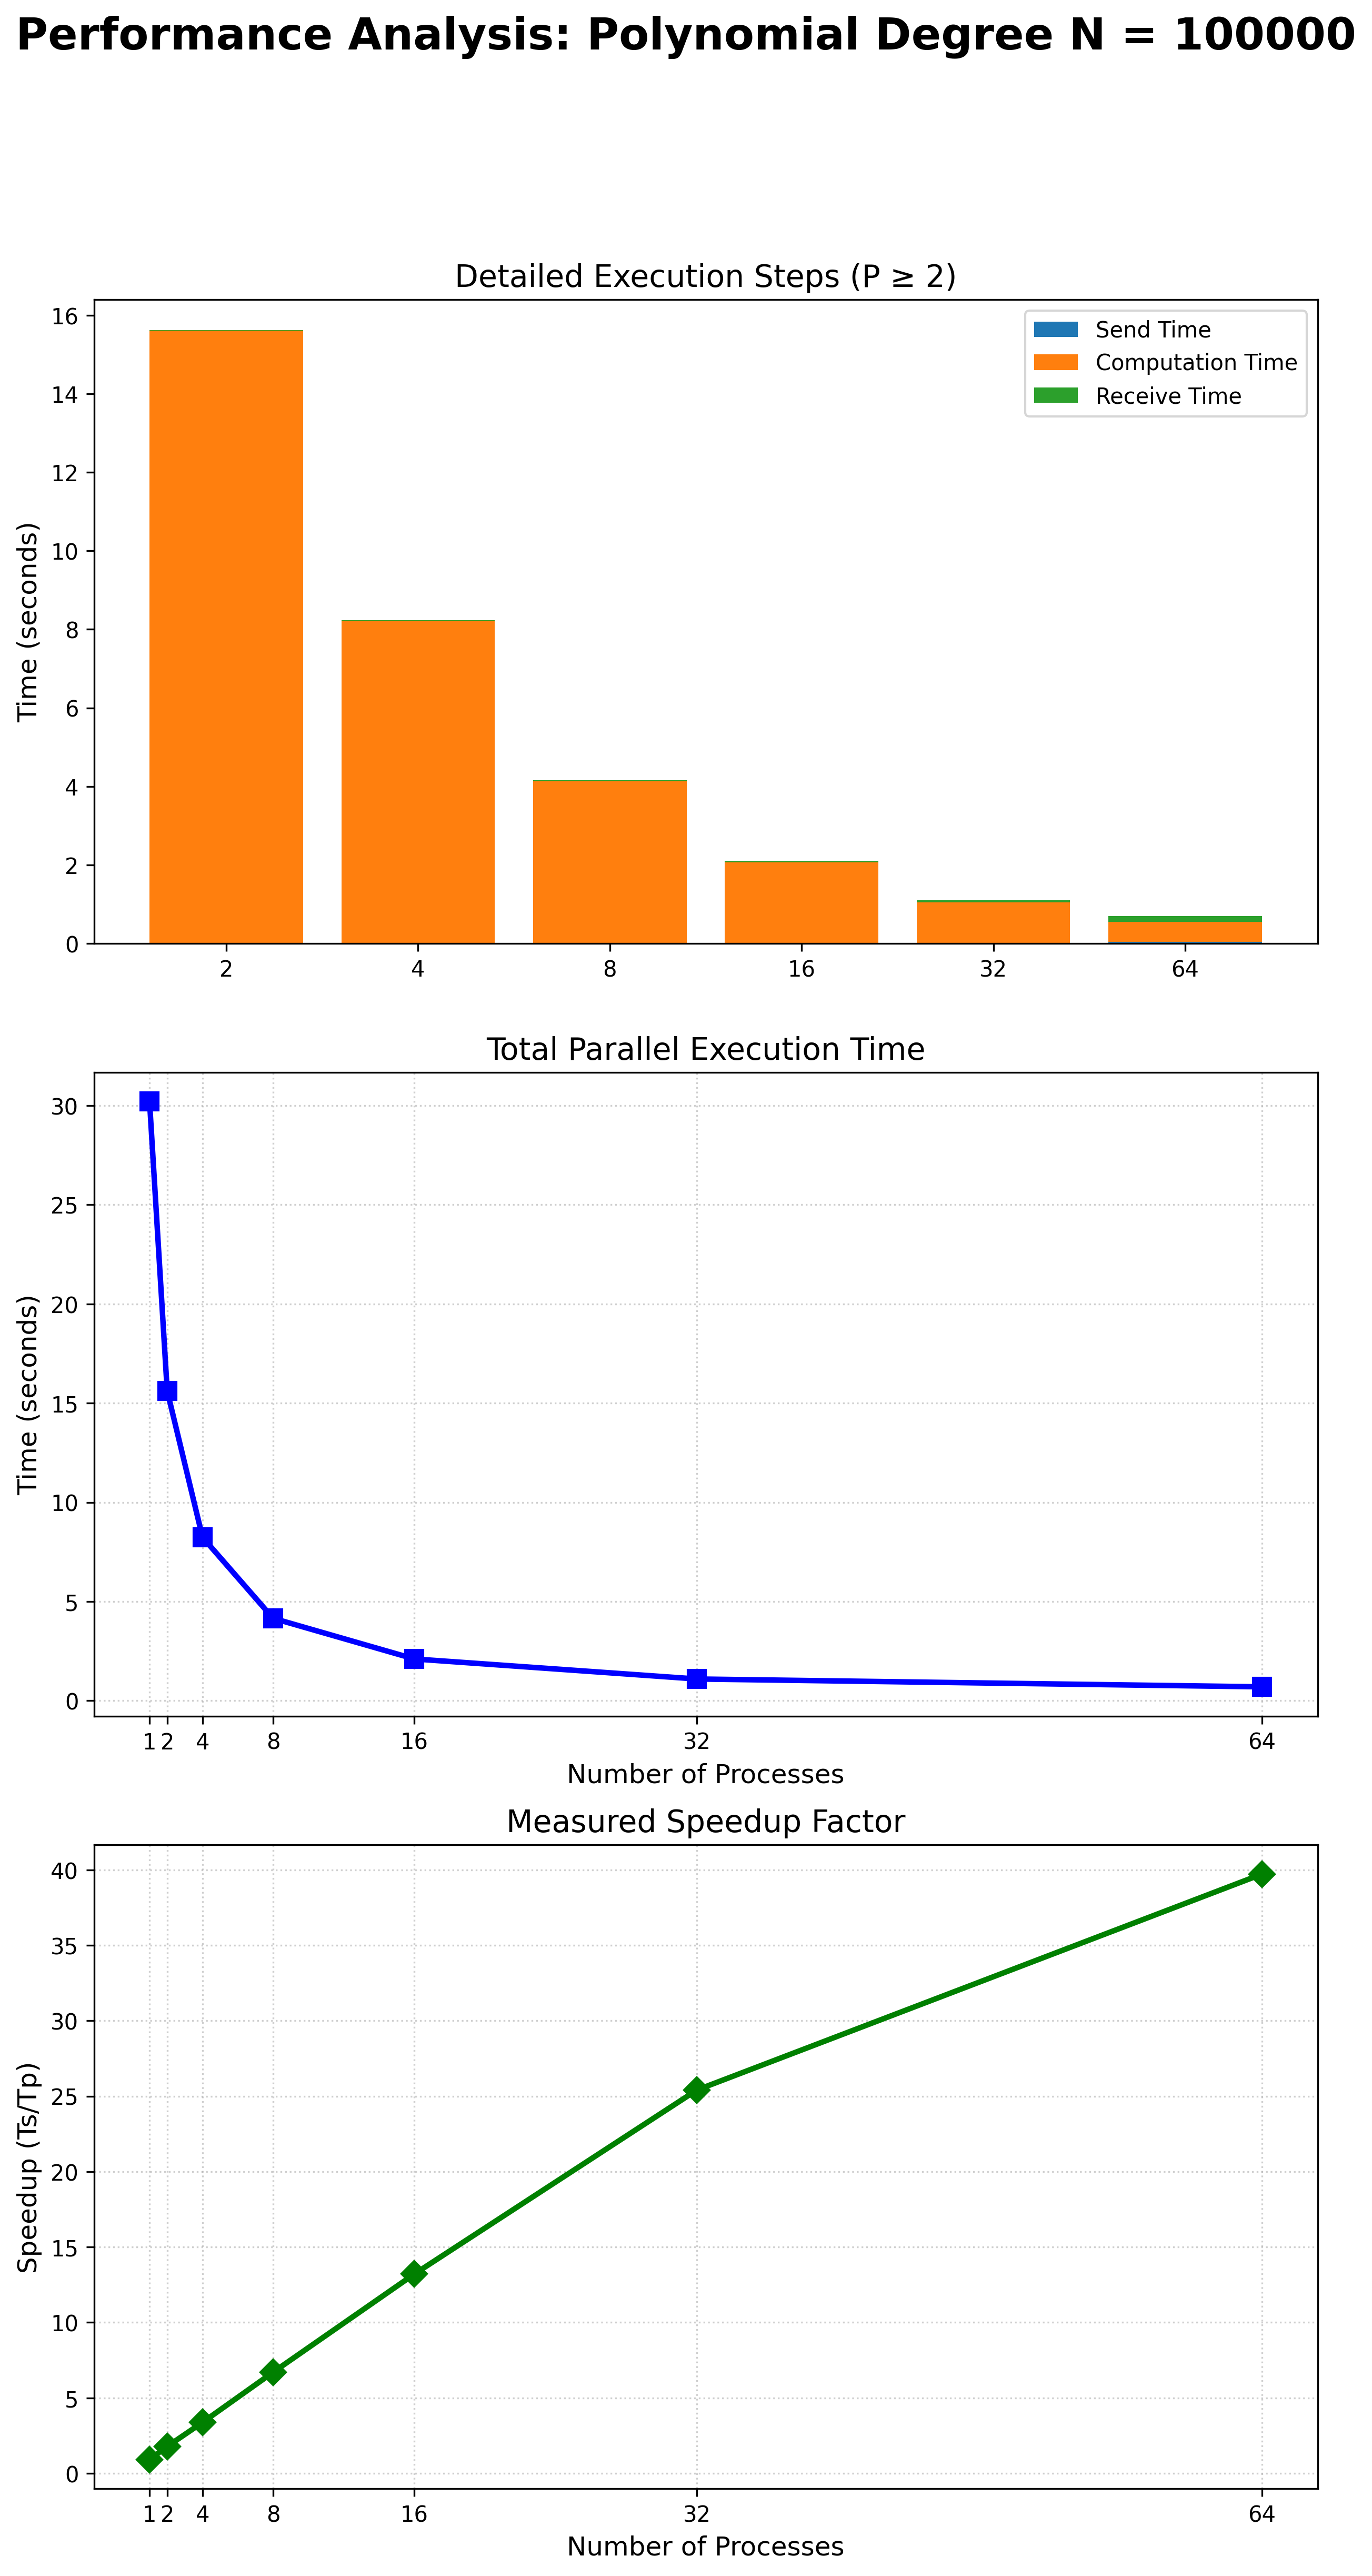
\includegraphics[width=0.8\linewidth]{graphs/pol_mult_N100000.png}
\end{figure}


\begin{figure}[htbp]
    \centering
    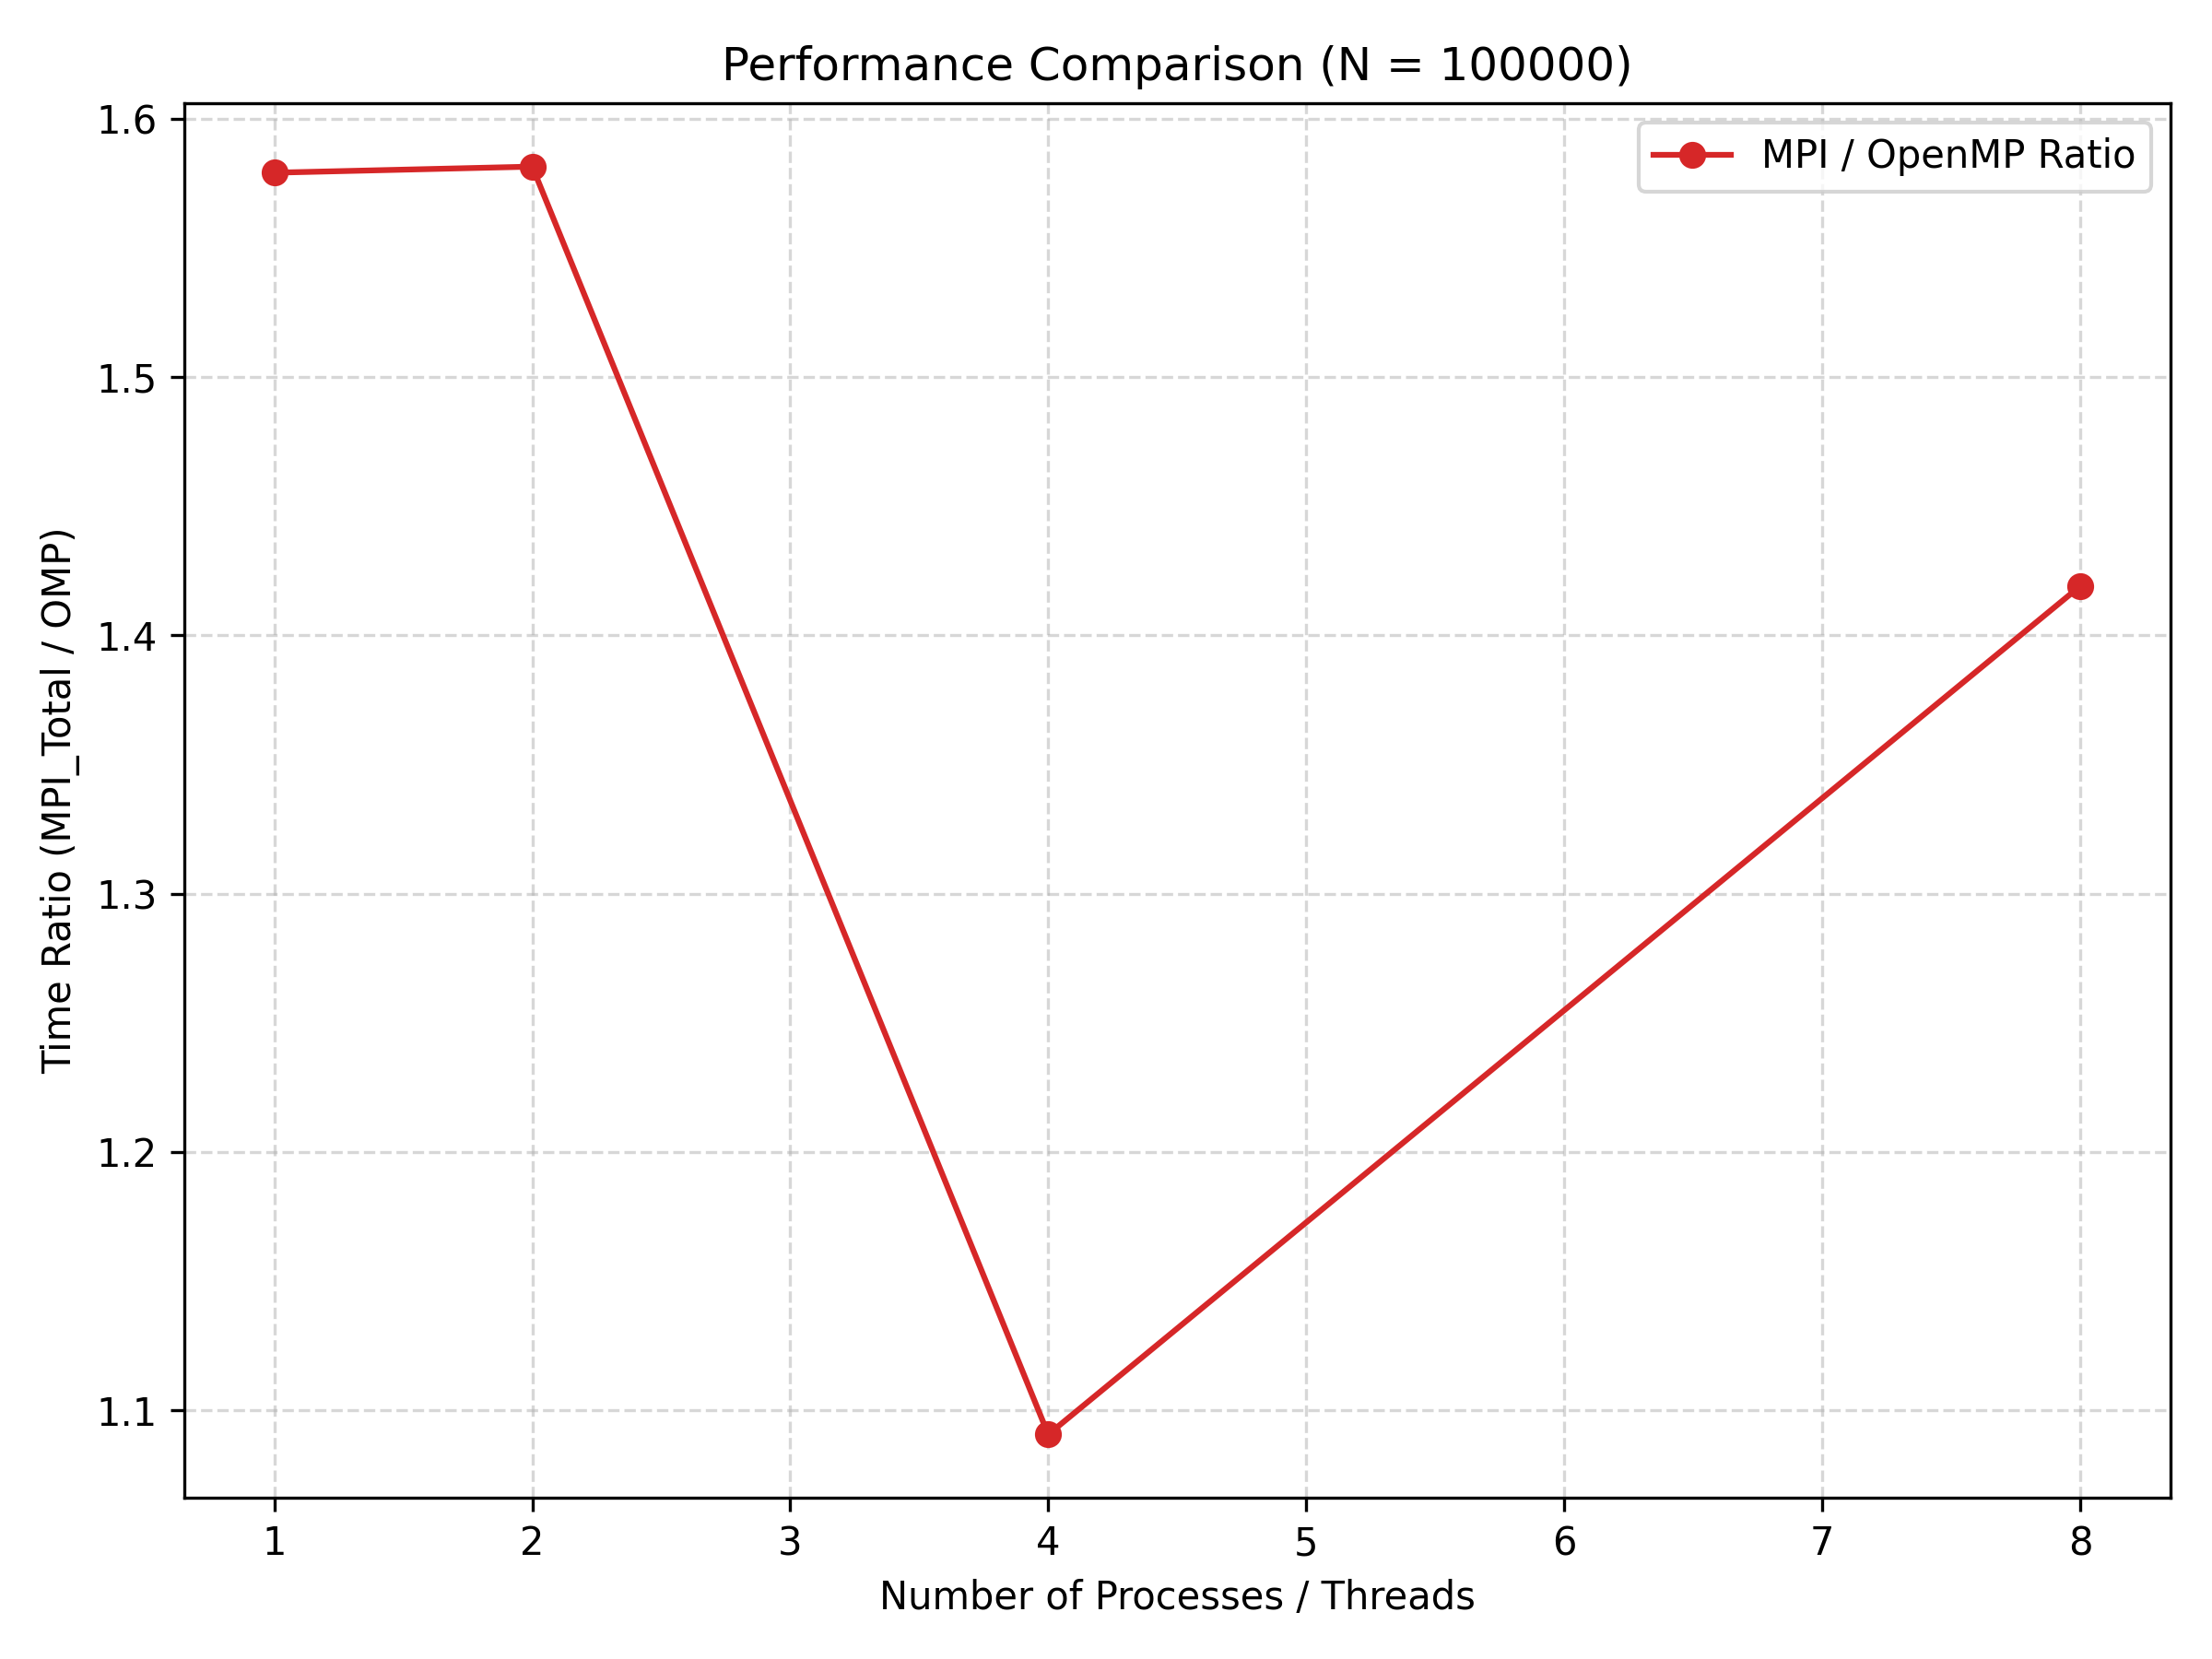
\includegraphics[width=0.8\linewidth]{graphs/mpi_vs_omp_N100000.png}
\end{figure}

\FloatBarrier
\underline{Συμπεράσματα}:
Για μικρά \en{n} και ειδικά όσο αυξάνεται ο αριθμός των διεργασιών ο περισσότερος χρόνος δαπανάται στην επικοινωνία
παρά στο κομμάτι του υπολογισμού. Άρα και η επιτάχυνση έναντι του σειριακόυ είναι περιορισμένη με μέγιστο να φτάνει το
$\sim$ 3.5 . Βέβαια μετά από κάποιο σημείο η αύξηση του αριθμού των διεργασιών βλάπτει πετυχαίνοντας χειρότερους χρόνους,
άρα και επιτάχυνση από τον σειριακό. Για μεγάλα \en{n}, ο χρόνος επικοινωνίας είναι αμελητέος μπροστά στο χρόνο υπολογισμού
και η επιτάχυνση μεγαλώνει και μεγιστοποιείται στο $\sim$ 40 σε σχέση με τον σειριακό για 64 διεργασίες.
Η υλοποίηση με \en{openmp} είναι πιο αποδοτική της \en{mpi} σε έναν κόμβο με μέγιστη επιτάχυνση (έναντι της \en{mpi})
$\sim$ 1.6. Αυτό γιατί στην υλοποίηση με νήματα δε χρειάζεται κάποια επικοινωνία μεταξύ τους αφού λειτουργόυν πάνω στα ίδια
δεδομένα. 
\FloatBarrier


\section{\en{Sparse Matrix-Vector Multiplication}}
Η δεύτερη άσκηση επικεντρώνεται στον αποδοτικό πολλαπλασιασμό πίνακα-διανύσματος με χρήση της
τεχνικής \en{CSR}. 
Η αρχικοποίηση γίνεται ως εξής:
Κρατούνται τέσσερις πίνακες: \en{values, col\_index, row\_index}.
Ο \en{values} κρατά τις μη μηδενικές τιμές του πίνακα με τη σειρά που διαβάζονται (ανά γραμμές).
Ο \en{col\_index} τις στήλες που αυτές οι τιμές βρίσκονται (με τη σειρά που εμφανίζονται στον \en{values}).
Ο \en{row\_index} πόσα στοιχεία είναι μη μηδενικά πάνω από τη γραμμή \en{i} (πχ \en{row\_index[2]} = πόσα μη
μηδενικά υπάρχουν πάνω από τη γραμμή 2).
Οι πίνακες του \en{CSR} όπως και ο κανονικός δημιουργούνται στη διεργασίας 0 σειριακά.
\newpage
\subsection{\en{Dense Compute}}
Ο κανονικός πίνακας σπάει ανά γραμμές. Επειδή μπορεί το \en{n} να μη διαιρείται με το πλήθος των διεργασιών (\en{num\_proc}),
χρησιμοποιούνται οι (\en{Scatterv, Gatherv, Allgtherv}) και υπολογίζονται οι πίνακες \en{sendocount, displacements}. Όπως και
πριν το υπόλοιπο (σε πλήθος γραμμών) μοιράζεται στα πακέτα γραμμών που δημιουργούνται. Ο υπολογισμός είναι ο κλασσικός, μόνο
που στο τέλος κάθε επανάληψης χρειάζεται το μερικό αποτέλεσμα που υπολογίζει κάθε διεργασία να πάει στις υπόλοιπες (\en{Allgetherv}).
Στη τελευταία, τα μερικά αποτελέσματα συγκεντρόνονται στη 0.
Ο χρόνος του παράλληλου υπολογισμού είναι το \en{max=\{execution time of proc i\}}.

\subsection{\en{Csr Compute}}
Μοιράζεται ο πίνακας \en{values} στις διεργασίες. Κάθε διεργασία παίρνει ένα πλήθος γραμμών που βρίσκεται πιο
κοντά στον $fair\_size = non\_zero / num\_proc$, δηλαδή αν βάζοντας και την επόμενη γραμμή του κανονικού πίνακα έχω
$\geq fair\_size$ τότε αυτές οι γραμμές (από το τελευταίο \en{split} μέχρι αυτή αποτελούν το πακέτο που θα πάει στη
διεργασία \en{i}). Αυτό γίνεται για εξισορρόπηση φορτίου, επειδή η κατανομή των μηδενικών στις γραμμές δεν είναι γνωστή.
Μάζι με τον πίνακα \en{values} μοιράζονται και οι \en{row/col\_index}. \en{Broadcast} γίνονται οι \en{sendcount,displacements}
πίνακες που χρειάζονται να συνοδεύουν το \en{scatter} που γίνεται στους πίνακες του \en{csr}.
Η υλοποίηση του πολλαπλασιασμού είναι ακριβώς όπως περιγράφεται στο: 
\en{\url{https://people.eecs.berkeley.edu/~aydin/csb2009.pdf}}.
Στο τέλος κάθε επανάληψης, χρησιμοποιείται όπως και στη \en{dense} περίπτωση \en{Gatherv,Allgatherv} ανάλογα με το αν είναι
η τελευταία επανάληψη ή όχι. Ο χρόνος του παράλληλου υπολογισμού είναι το \en{max=\{execution time of proc i\}}.
\\
\en{\runcmd{mpiexec -n <num\_proc> ./sparse -n <matrix size> -p <sparsity:0-100> -i <iterations>}}

\underline{Σημείωση}: 
Όλα τα πειράματα υπάρχουν και στο \en{csv} αρχείο: \en{benchmarks\_sparse.csv}.
Τα παρακάτω διαγράμματα προβάλλουν κάποια αποτελέσματα για δεδομένες τιμές των 
άλλων παραμέτρων (που επιλέχθηκαν για να αναδεικνύουν την υπεροχή του \en{CSR}).

\begin{figure}[htbp]
    \centering
    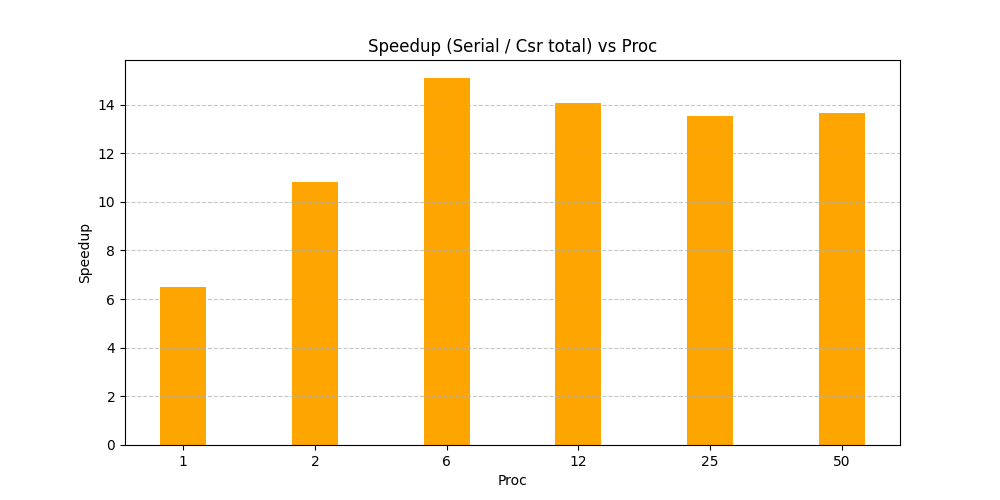
\includegraphics[width=0.8\linewidth]{graphs/speedup_vs_proc_csr_total_bar.png}
    \caption{\en{Speedup vs procs: n=10000, sparsity=90, iter=70}}
    \label{fig:total}
\end{figure}

\begin{figure}[htbp]
    \centering
    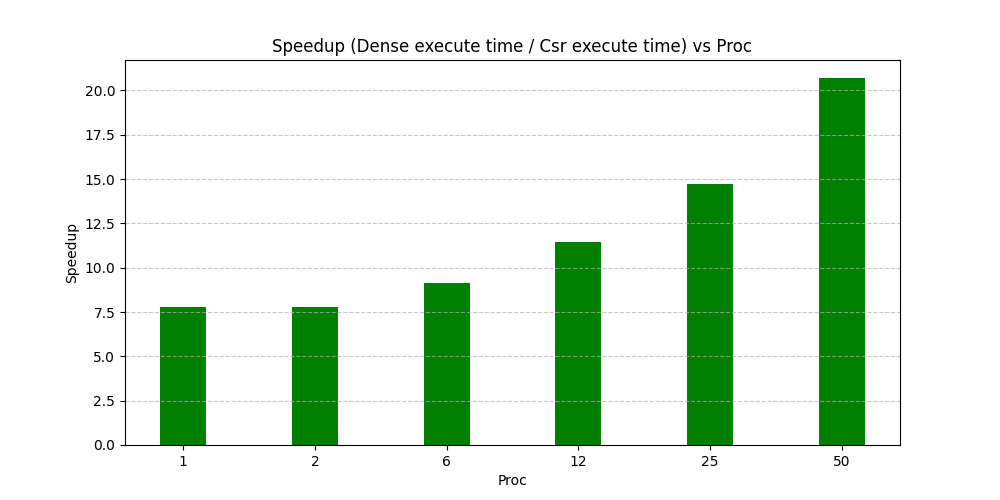
\includegraphics[width=0.8\linewidth]{graphs/speedup_dense-ex_csr-ex_bar.png}
    \caption{\en{Speedup vs procs: n=10000, sparsity=90, iter=70}}
    \label{fig:pure_execute}
\end{figure}

\begin{figure}[htbp]
    \centering
    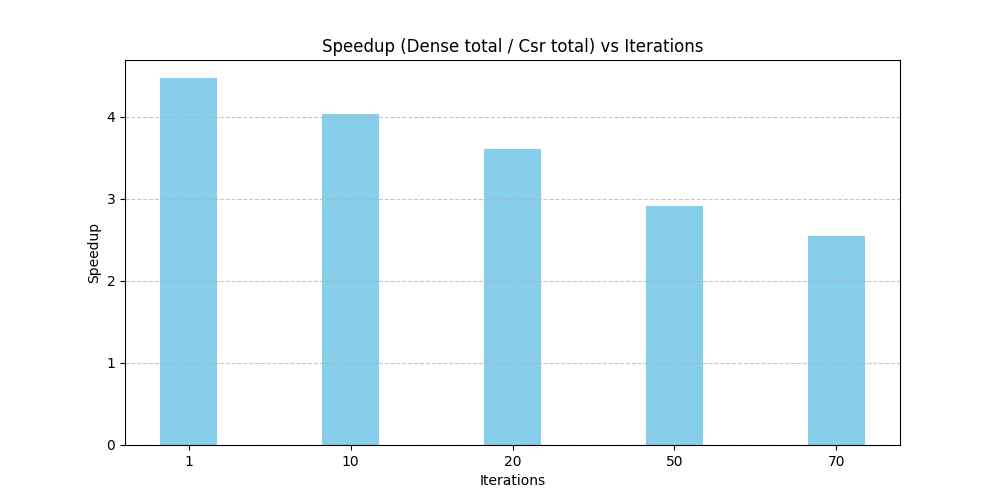
\includegraphics[width=0.8\linewidth]{graphs/speedup_vs_iterations_dense-csr_total_bar.png}
    \caption{\en{Speedup vs iterations: n=10000, sparsity=90, proc=50}}
    \label{fig:iterations}
\end{figure}

\begin{figure}[htbp]
    \centering
    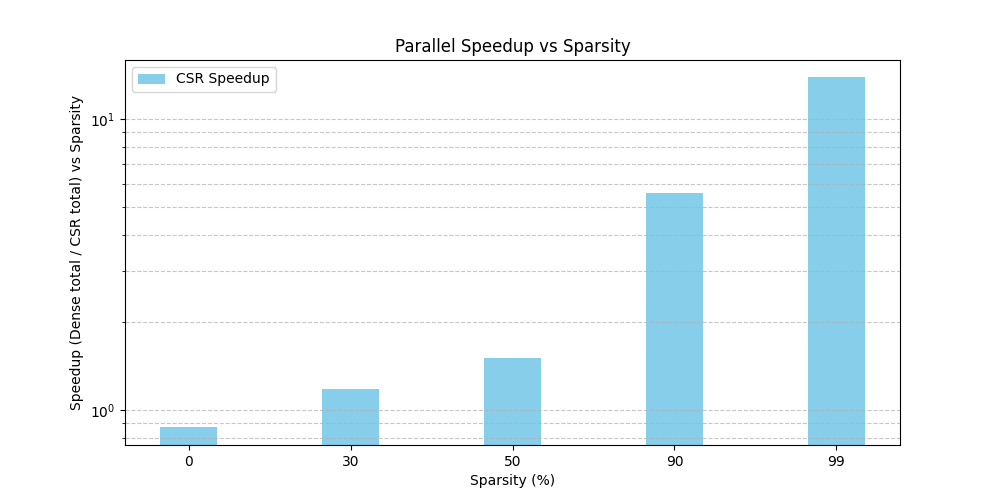
\includegraphics[width=0.8\linewidth]{graphs/speedup_vs_sparsity_dense-csr_total_bar.png}
    \caption{\en{Speedup vs sparsity: n=10000, iter=70, proc=50}}
    \label{fig:sparsity}
\end{figure}

\FloatBarrier
\underline{Συμπεράσματα}:
Η επιτάχυνση του \en{CSR} σε σχέση με τον σειριακό αλγόριθμο είναι μεγάλη σε υψηλά \en{sparsity} και
μεγαλύτερους σε μέγεθος πίνακες. Η στασιμότητα στην επιτάχυνση ($\sim 14$ για 12,25,50 διεργασίες) οφείλεται
στον παραπάνω χρόνο επικοινωνίας που χρειάζεται καθώς αυξάνονται (επίσης όσα περισσότερα μηχανήματα δεσμεύονται,
τόση μεγαλύτερη η πιθανότητα χρησιμοποιηθεί ένα ή περισσότερα που δεν είναι αδρανή).
Καθώς αυξάνεται το \en{sparsity} και για αρκούντως μεγάλους πίνακες,
το \en{CSR} υπερτερεί του απλού παράλληλου αλγορίθμου, αφού παραλείπονται οι ανούσιοι πολλαπλασιασμοί
πετυχαίνοντας μέγιστη επιτάχυνση (έναντι αυτού) $\sim 14$.
Η αύξηση του αριθμού των επαναλήψεων μειώνει την επιτάχυνση του \en{Csr} έναντι του \en{Dense} 
($\sim 4$ στις 10, $\sim 2.5$ στις 70). Αυτό γιατί η επικοινωνία που χρειάζεται σε κάθε επανάληψη (\en{gatherv}),
αρχίζει να γίνεται αισθητή καθώς αυξάνονται οι επαναλήψεις.
Κοιτώντας μόνο το χρόνο υπολογισμού, η \en{Csr} υπερτερεί της \en{Dense} υλοποίησης και μάλιστα πετυχαίνοντας 
\en{max} επιτάχυνση: $\sim 21$. Προφανώς αυτό παρατηρείται επειδή η \en{Csr} αποφεύγει μη αναγκαίες πράξεις. 

\section{\en{Hybrid Sparse Matrix-Vector Multiplication}}
Η τρίτη άσκηση επεκτείνει τη 2η, προσθέτοντας την ικανότητα της χρήσης \en{Openmp} για τη δουλειά που έχει
να κάνει κάθε διεργασία. Προστέθηκαν οι εντολές για \en{openmp} στο ίδιο αρχείο \en{sparse\_mat\_vec.c} με \en{guards}.
Στις συναρτήσεις που υπολογίζεται ο πολλαπλασιασμός, δημιουργείται ένα \en{parallel block} και παραλληλοποιείται η 
εκτέλεση του πολλαπλασιασμού. Στο τέλος κάθε επανάληψης ένα από τα νήματα είναι υπεύθυνο να καλέσει τη \en{allgatherv,gatherv}.
\\
\en{\runcmd{mpiexec -n <proc> ./hybrid\_sparse -n <matrix size> -p <sparsity:0-100> -i <iter> -t <thr>}}

\underline{Σημείωση}: 
Τα πειράματα υπάρχουν και στο \en{csv} αρχείο: \en{hybrid\_comparison.csv}.

\begin{figure}[htbp]
    \centering
    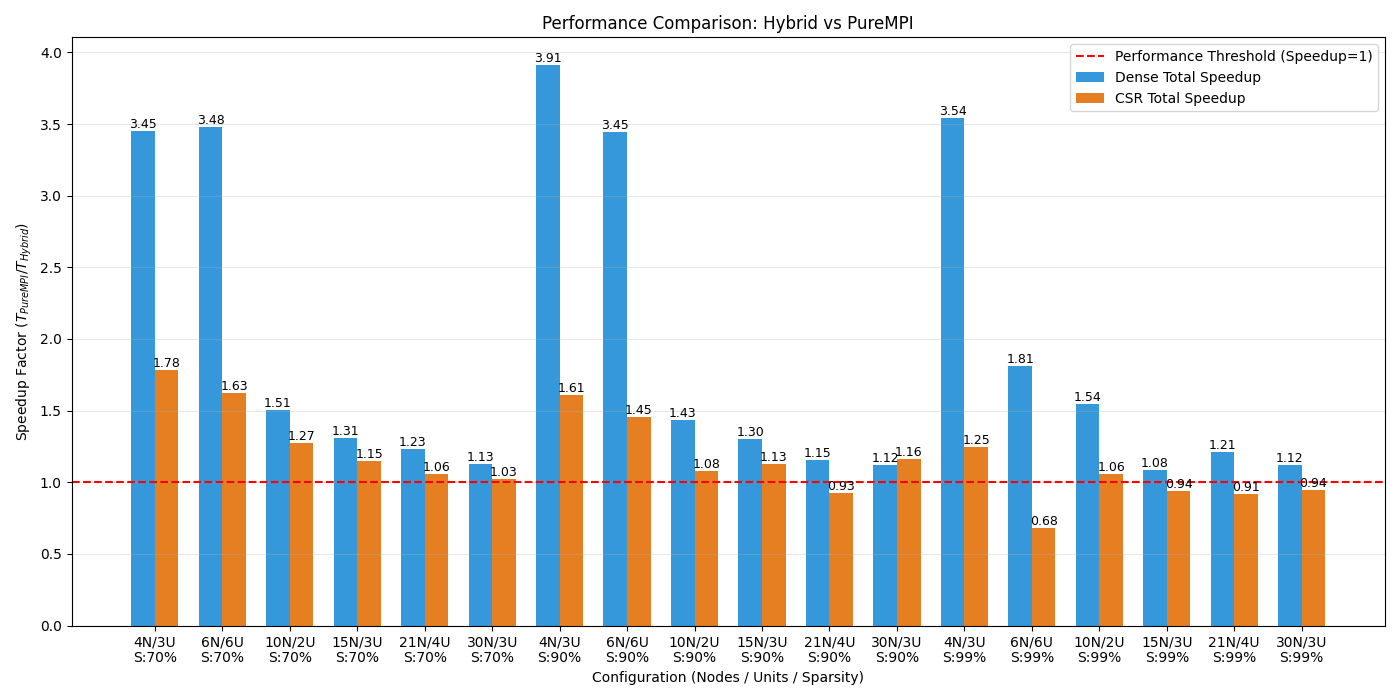
\includegraphics[width=0.8\linewidth]{graphs/hybrid_vs_purempi_comparison.png}
    \caption{\en{Speedup (mpi / hybrid), N=20000}}
\end{figure}

\FloatBarrier
\underline{Συμπεράσματα}:
Το κέρδος από την \en{hybrid} υλοποίηση είναι περιορισμένο (όπως φαίνεται και στο διάγραμμα).
Υπάρχει μια βελτίωση ($\sim 3.5-4$) όταν χρησιμοποιούνται 4/6 κόμβοι, ενώ στις υπόλοιπες
περιπτώσεις κινείται στους ίδιους χρόνους με την \en{pure mpi} υλοποίηση. Το αναμενόμενο ήταν να συμφέρει
η \en{Openmp} γενικά, λόγω του μειωμένου συνολικού αριθμού διεργασιών σε σχέση με την \en{pure mpi} άρα και
επικοινωνίας στη κάθε επανάληψη. Ίσως επιβαρύνει και το \en{runtime} της \en{openmp}. 




\end{document}